\subsection{Αλγόριθμός Εξίσωσης Ευθείας}
Για παράδειγμα θα μπορούσαμε να χρησιμοποιήσουμε την αλγεβρική εξίσωση της ευ θείας για να προσδιορίσουμε ποια σημεία της ευθείας θα αντιστοιχούν σε pixel της οθόνης που θα επιλέξουμε να φωτίσουμε.

Αν θέλουμε να σχεδιάσουμε το ευθύγραμμο τμήμα $\olsi{P_1 P_2}$, με $P_1 = 
(x_1, y_1)$ και $P_2 = (x_2, y_2)$, τότε θα ισχύει:

\begin{equation*}
	\cfrac{y-y_1}{x-x_1} = \cfrac{y_2-y_1}{x_2-x_1} \Rightarrow y = \cfrac{y_2-y_1}{x_2-x_1}x + \cfrac{y_1x_2-y_2x_1}{x_2-x_1}
\end{equation*}
Θέτοντας, $S = \cfrac{y_2-y_1}{x_2-x_1}$ (κλίση) και $C = \cfrac{y_1x_2-y_2x_1}{x_2-x_1}$, προκύπτει ότι: $y=Sx+c$. Με βάση αυτή την εξίσωση, γράφουμ τον ακόλουθο αλγόριθμό:


\textbf{\underline{Βήμα 1:}} Διάβασε $P_1 = (x_1, y_1)$ και $P_2 = (x_2, y_2)$. \newline 
\textbf{\underline{Βήμα 2:}} Υπολόγισε $S = \cfrac{y_2-y_1}{x_2-x_1}$ (κλίση) και $C = \cfrac{y_1x_2-y_2x_1}{x_2-x_1}$. \newline 
\textbf{\underline{Βήμα 3:}} Για $x$ από $x_1$ έως $x_2$ με βήμα 1, υπολόγισε το $y = round(Sx+C)$ και φώτισε το pixel $(x,y)$. 
	
\begin{lstlisting}[caption={Plot Line Algorithm}]
function (x1, y1, x2, y2)
	if x1 == x2
		x = x1
		for y= y1:y2
			plot(x,y)
        end    
        return
	end	
    
    # Compute the slope
    s = (y2-y1)/(x2-x1)
    
    c = (y1x2-y2x1)/ (x2-x1)
    for x= x1:x2
    	y = round(sx +c)
    	plot(x,y)
    end    
end
\end{lstlisting}

Παρατηρούμε ότι ο αλγόριθμος έχει μικρή απαιτεί 1 flop για κάθε σημείο που θα εμφανιστεί στην οθόνη συντεταγμένη. Τα σημεία αυτά θα είναι όσα η διαφορά των τετμημένων των 2 σημείων μεταξύ των οποίων θέλουμε να σχηματίσουμε την ευθεία.

\begin{application}[Εφαρμογή του αλγορίθμου plot-line]
		Να εφαρμοστεί ο αλγόριθμος plot-line για τα ζεύγη σημείων:
\begin{enumerate}
	\item[$\mathrm{i)}$] $P_1 = (1, 1), P_2 = (3, 2)$
	\item[$\mathrm{ii)}$] $P_1 = (1, 1), P_2 = (4, 13)$
	\item[$\mathrm{iii)}$] $P_1 = (0, 0), P_2 = (0, 10)$	
\end{enumerate}

\begin{solution}
		

\begin{enumerate}
	\item[$\mathrm{i)}$] $P_1 = (1, 1), P_2 = (3, 2)$ \newline 
		\textbf{\underline{Βήμα 1}} (Υπολογισμός $s$):	
		\[
		s = \frac{y_2 - y_1}{x_2 - x_1} = \frac{2 - 1}{3 - 1} = \frac{1}{2} = 0.5
		\] 	
		
		\textbf{\underline{Βήμα 2}} (Υπολογισμός $c$):	
		\[
		c = \frac{y_1 x_2 - y_2 x_1}{x_2 - x_1} = \frac{1 \cdot 3 - 2 \cdot 1}{3 - 1} = \frac{3 - 2}{2} = \frac{1}{2} = 0.5	
		\]
		\textbf{\underline{Βήμα 3}} (Υπολογισμός και φωτισμός σημείων):		
		\begin{align*}
		   \text{For } x = 1: & \quad y = \text{round}(0.5 \cdot 1 + 0.5) = \text{round}(1) = 1 \\
		   \text{For } x = 2: & \quad y = \text{round}(0.5 \cdot 2 + 0.5) = \text{round}(1.5) = 2 \\
		   \text{For } x = 3: & \quad y = \text{round}(0.5 \cdot 3 + 0.5) = \text{round}(2) = 2 \\
		\end{align*}
		Άρα συνολικά θα φωτιστούν τα σημεία: \( (1, 1), (2, 2), (3, 2) \).
		
		\begin{figure}[hbt]
		  \begin{center}
			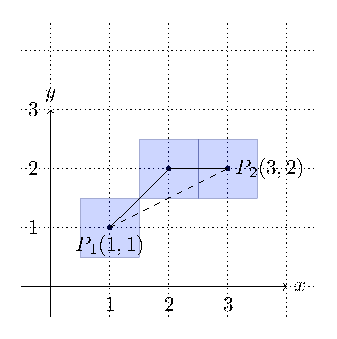
\includegraphics[scale=1]{Chapter1/Plot-Line/application1a.pdf}
		  \end{center}
		  \caption{Φωτισμένα σημεία έπειτα από εφαρμογή αλγορίθμου Plot Line για τα σημεία $P_1 = (1,1), P_2 = (3,2)$}
		\end{figure}


	\item[$\mathrm{ii)}$] $P_1 = (1, 1), P_2 = (4, 13)$ \newline 
		\textbf{\underline{Βήμα 1}} (Υπολογισμός $s$):
		\[
		   s = \frac{13 - 1}{4 - 1} = \frac{12}{3} = 4
		\]
		
		\textbf{\underline{Βήμα 2}} (Υπολογισμός $c$):
		   \[
		   c = \frac{1 \cdot 4 - 13 \cdot 1}{4 - 1} = \frac{4 - 13}{3} = \frac{-9}{3} = -3
		   \]
		
		\textbf{\underline{Βήμα 3}} (Υπολογισμός και φωτισμός σημείων):	
		   \begin{align*}
		   \text{For } x = 1: & \quad y = \text{round}(4 \cdot 1 - 3) = \text{round}(1) = 1 \\
		   \text{For } x = 2: & \quad y = \text{round}(4 \cdot 2 - 3) = \text{round}(5) = 5 \\
		   \text{For } x = 3: & \quad y = \text{round}(4 \cdot 3 - 3) = \text{round}(9) = 9 \\
		   \text{For } x = 4: & \quad y = \text{round}(4 \cdot 4 - 3) = \text{round}(13) = 13 \\
		   \end{align*}
		Άρα συνολικά θα φωτιστούν τα σημεία: \( (1, 1), (2, 5), (3, 9), (4, 13) \).	
	
	\item[$\mathrm{iii)}$]  \( P_1 = (0, 0), P_2 = (0, 10) \) \newline 
		Εφόσον τα σημεία $P_1, P_2$ έχουν την ίδια τετμημένη, τότε θα σχεδιάσουμε την κάθετη γραμμή που τα ενώνει. 	
		Άρα συνολικά θα φωτιστούν τα σημεία: $ (0, 0), (0, 1), (0, 2), \ldots, (0, 10) $.
		
		\begin{figure}[h!]
			\begin{minipage}[b]{0.48\textwidth} % Top-left image	
				\begin{center}
				    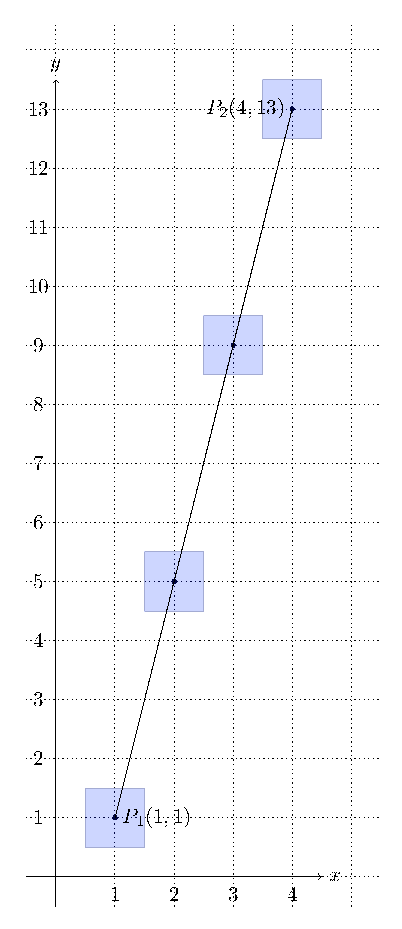
\includegraphics[scale=0.7]{Chapter1/Plot-Line/application1b.pdf}
				\end{center}    
			\end{minipage}%
			\hfill
			\begin{minipage}[b]{0.48\textwidth} % Top-right image
			    \begin{center}
				    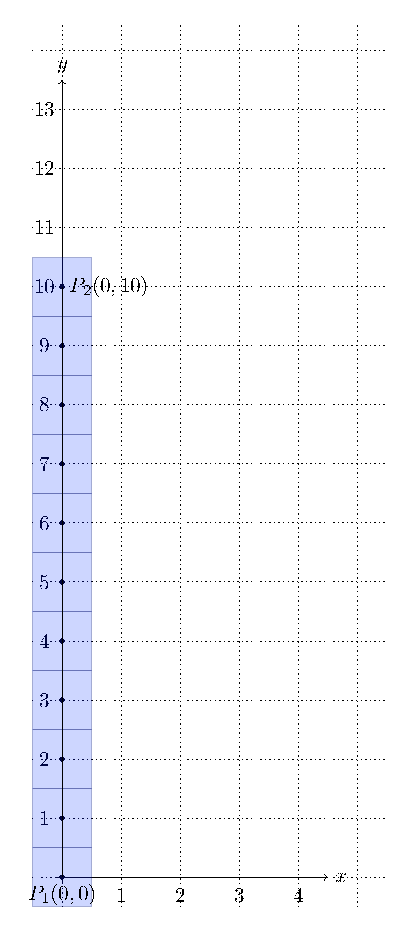
\includegraphics[scale=0.7]{Chapter1/Plot-Line/application1c.pdf}
				\end{center}    
			\end{minipage}
			\caption{Φωτισμένα σημεία έπειτα από εφαρμογή αλγορίθμου Plot Line για τα σημεία $P_1 = (1,1), P_2 = (3,2)$}
		\end{figure}

\end{enumerate}


\end{solution}
	
\end{application}

\subsection{Μειονεκτήματα Αλγορίθμου εξίσωσης ευθείας}

Αν χρησιμοποιήσουμε αυτόν τον αλγόριθμο θα παρατηρήσουμε ότι για ζεύγη σημείων το ευθύγραμμο τμήμα μας θα παρουσιάζει κενά και δεν θα είναι συνεχές.

Συγκρεκριμένα, αν η κλίση είναι μεγαλύτερη του $1$, τότε ο αλγόριθμος δε φωτίζει συνεχόμενα pixel.
Αυτό το πρόβλημα, μπορεί να διορθωθεί, εκφράζοντας το $x$ σα συνάρτηση του $y$.

\[
	x = f(y) = \cfrac{x_2 - x_1}{y_2- y_1}y +  \cfrac{ y_2 x_1 - y_1 x_2  }{ y_2 - y_1 } 
\]

 Επίσης κατά τον υπολογισμό των τιμών πραγματοποιούμε πολλαπλασιασμούς και διαιρέσεις που αυξάνουν την πολυπλοκότητα και εισάγουν και αριθμητικά σφάλματα στα δεδομένα μας. Κάθε σημείο απαιτεί για τον υπολογισμό του \texttt{1 flop + 1 rounding}, άρα η πολυπλοκότητα του αλγορίθμου είναι αυξημένη.
 
 Για αυτούς τους λόγους η χρήση της αλγεβρικής εξίσωσης της ευθείας σε υπολογιστή δεν είναι βέλτιστη. Ευτυχώς έχουν ήδη αναπτυχθεί άλλοι τρόποι που θα μας βοηθήσουν να υπολογίσουμε ποια πιξελ θα πρέπει να φωτίσουμε στην οθόνη για να σχηματιστεί το ζητούμενο ευθύγραμμο τμήμα. Ένα τέτοιος είναι ο αλγόριθμος ευθυγράμμων τμημάτων του Bresenham.

